\documentclass[crop=false,10pt]{standalone}
\usepackage{standard}

\begin{document}
  \section{The Model} % (fold)
  \label{sec:The Model}
    \begin{figure}
      \center
      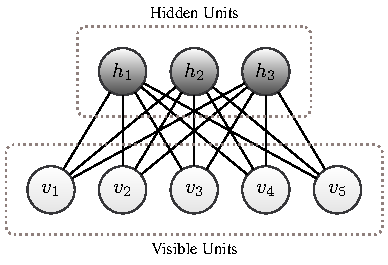
\includegraphics[width=0.9\textwidth]{figures/rbm-scheme-inputs.pdf}
      \caption{%
        The figure shows the basic scheme of an RBM with the separated hidden and visible values.
      }
      \label{fig:rbm-scheme-inputs}
    \end{figure}
    \begin{figure}
      \center
      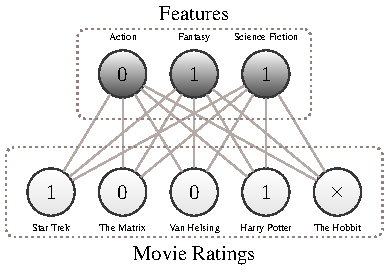
\includegraphics[width=0.9\textwidth]{figures/rbm-scheme-example.pdf}
      \caption{%
        The figure shows the basic scheme of an RBM applied to the example of movie ratings from a user.
      }
      \label{fig:rbm-scheme-example}
    \end{figure}
    \begin{figure}
      \center
      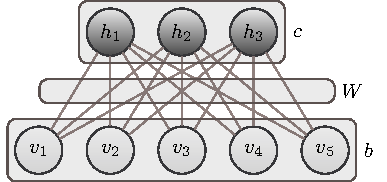
\includegraphics[width=0.9\textwidth]{figures/rbm-scheme.pdf}
      \caption{%
        The figure shows the basic scheme of an RBM with the weight matrix $W$ and bias vectors $b$ and $c$ as parameters describing the probability distribution modelled by the RBM.
      }
      \label{fig:rbm-scheme-example}
    \end{figure}
    \[
      v \in V \define \set{0,1}{}^n
      \separate
      h \in H \define \set{0,1}{}^m
      \separate
      ϑ \define (W,b,c) \in \setReal^{(n\times m) + n + m}
    \]
    \[
      \function{p[ϑ]}{V\times H}{[0,1]}
      \separate
      p[ϑ](v,h) \define \frac{e^{ -E[ϑ](v,h) }}{Z(ϑ)}
    \]
    \[
      \function{E[ϑ]}{V\times H}{\setReal}
      \separate
      E[ϑ](v,h) \define -\transpose{v}Wh - \transpose{v}b - \transpose{h}c
    \]
    \[
      Z(ϑ) \define \sum_{v\in V} \sum_{h\in H} e^{ -E[ϑ](v,h) }
    \]
    \[
      \function{p[ϑ]}{V}{[0,1]}
      \separate
      p[ϑ](v) \define \sum_{h\in H} p[ϑ](v,h)
    \]
    \[
      p[ϑ](h \vert v) = \prod_{j=1}^m p[ϑ]\roundBrackets{h_j=1 \middle\vert v}
    \]
  % section The Model (end)
\end{document}